\section{Expanders}

The Exander Framework allows for the miscellaneous execution of expanders of any type. The
Expander Framework is independent of any of the details of Expanders, fully adhering to
the principle of \gls{dip}. Conversely, an Expander is required to implement several
interfaces to ensure execution and dependency management are available during runtime. The
Expander Framework also consists of a set of default tasks, such as the execution of the
expansion tasks known as ExpanderHandlerInteractors
\citecode{koks_iexpanderhandlerinteractor_2023}, logging, bootstrapping dependencies, and
tasks to execute harvestings and injections. Except for the use of the
IExpanderInteractor, non of which are required.

Figure \ref{fig_expander_design} illustrates the dependencies between the domain layer of
the Expander Framework. The Clean Architecture Expander is considdered to operate as an
application layer, which contain specific tasks bounded to a particular application or
process. In this case the Expansion process.

\begin{figure}[H]
    \centering
    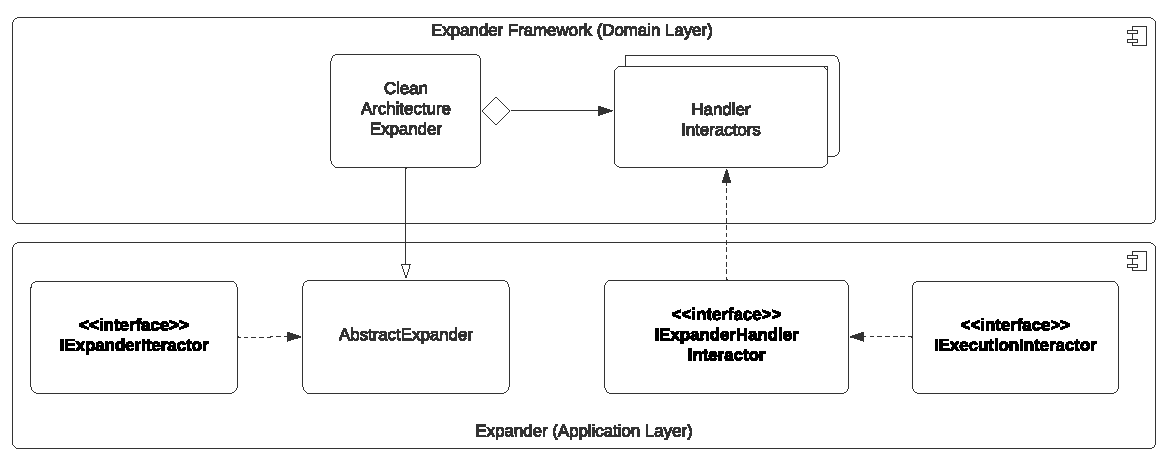
\includegraphics[width=1\textwidth]{figures/expander.pdf}
    \caption[The Design of an Expander]{The Design of an Expander}
    \label{fig_expander_design}
  \end{figure}